%% For normal draft builds (figs undisplayed hence fast compile)
%\documentclass[hyperpdf,nobind,draft,oneside]{hepthesis}
%\documentclass[hyperpdf,nobind,draft,twoside]{hepthesis}

%% For short draft builds (breaks citations by necessity)
%\documentclass[hyperpdf,nobind,draft,hidefrontback]{hepthesis}

%% For Cambridge soft-bound version
%\documentclass[hyperpdf,bindnopdf]{hepthesis}
%% For Cambridge hard-bound version (must be one-sided)
\documentclass[hyperpdf,oneside]{hepthesis}

%% Load special font packages here if you wish
%\usepackage{lmodern}
\usepackage{mathpazo}
%\usepackage{euler}

\newcommand*{\BASEPATH}{./}

%% Put package includes etc. into preamble.tex for convenience
\usepackage{xspace}
\usepackage{tikz}
\usepackage{morefloats,subfig,afterpage}
\usepackage{mathrsfs} % script font
\usepackage{verbatim}
\usepackage{cite}
%\usepackage{float} #For demanding figure is placed exactly where specified using H 
%\usepackage{multirow} #For multi-row tables 

%% Using Babel allows other languages to be used and mixed-in easily
%\usepackage[ngerman,english]{babel}
\usepackage[english]{babel}
\selectlanguage{english}

\graphicspath{{\BASEPATH figures/}{\BASEPATH tables/}}

%% High-energy physics stuff
%\usepackage{abhep}
\usepackage{hepnames}
\usepackage{hepunits}

% Definitely useful JJ macros
\usepackage{\BASEPATH JJthesis-defs}

%Tell TexCount to track red text seperately
%TC:newcounter RedText Problem Text
%TC:macro \col [RedText]

%Tell TexCount how to correctly account for macros: \macro #Words
%TC:macroword \ATLAS 1
%TC:macroword \ttbar 1
%TC:macroword \wdecay 2
%TC:macroword \wboson 2
%TC:macroword \mtop 1
%TC:macroword \mtopjet 2
%TC:macroword \zmumu 2
%TC:macroword \ljets 2
%TC:macroword \lpt 1
%TC:macroword \hpt 1
%TC:macroword \etmiss 1
%TC:macroword \HLTtap 1
%TC:macroword \frtwo 3
%TC:macroword \ISR 1
%TC:macroword \FSR 1
%TC:macroword \JSF 1
%TC:macroword \NDF 1
%TC:macroword \JSFdata 1
%TC:macroword \JSFsyst 1
%TC:macroword \JSFdatastat 1
%TC:macroword \jvt 1
%TC:macroword \nominal 2
%TC:macroword \mcatnlo 1
%TC:macroword \mcatnloX 1
%TC:macroword \phseven 2
%TC:macroword \AF 1
%TC:macroword \MC 1
%TC:macroword \RC 1
%TC:macroword \powheg 1
%TC:macroword \powhegbox 1
%TC:macroword \herwig 1
%TC:macroword \herwigseven 1
%TC:macroword \pythia 1
%TC:macroword \pythiasix 1
%TC:macroword \sherpa 1
%TC:macroword \evtgen 1
%TC:macroword \hathor 1
%TC:macroword \mgamc 1
%TC:macroword \madspin 1
%TC:macroword \openloops 1
%TC:macroword \openloopstwo 1
%TC:macroword \sherpaopenloops 2
%TC:macroword \mur 1
%TC:macroword \muf 1
%TC:macroword \muq 1
%TC:macroword \ttV 1
%TC:macroword \pThad 1
%TC:macroword \pTlep 1
%TC:macroword \pTttbar 1
%TC:macroword \HTfull 1
%TC:macroword \HTttbar 1
%TC:macroword \yhad 1
%TC:macroword \ylep 1
%TC:macroword \yttbar 1
%TC:macroword \mttbar 1
%TC:macroword \Naddjets 1
%TC:macroword \pTlead 1
%TC:macroword \pTsublead 1
%TC:macroword \dphileadhadtop 1
%TC:macroword \dphisubleadhadtop 1
%TC:macroword \dphilepbhadtop 1
%TC:macroword \dphittbar 1
%TC:macroword \dphileadsublead 1
%TC:macroword \mleadhadtop 1
%TC:macroword \Rleadhadtop 1
%TC:macroword \Rsubleadhadtop 1
%TC:macroword \arXivCode 1
%TC:macroword \CP 1
%TC:macroword \CPviolation 1
%TC:macroword \LHCb 1
%TC:macroword \LHC 1
%TC:macroword \LEP 1
%TC:macroword \CERN 1
%TC:macroword \bphysics 1
%TC:macroword \bhadron 1
%TC:macroword \Bmeson 1
%TC:macroword \bbaryon 1
%TC:macroword \Bdecay 1
%TC:macroword \bdecay 1



% Potentially useful Andy macros
% \DeclareRobustCommand{\parenths}[1]{\mymath{\left({#1}\right)}\xspace}
% \DeclareRobustCommand{\braces}[1]{\mymath{\left\{{#1}\right\}}\xspace}
% \DeclareRobustCommand{\angles}[1]{\mymath{\left\langle{#1}\right\rangle}\xspace}
% \DeclareRobustCommand{\sqbracs}[1]{\mymath{\left[{#1}\right]}\xspace}
% \DeclareRobustCommand{\mods}[1]{\mymath{\left\lvert{#1}\right\rvert}\xspace}
% \DeclareRobustCommand{\modsq}[1]{\mymath{\mods{#1}^2}\xspace}
% \DeclareRobustCommand{\dblmods}[1]{\mymath{\left\lVert{#1}\right\rVert}\xspace}
% \DeclareRobustCommand{\expOf}[1]{\mymath{\exp{\!\parenths{#1}}}\xspace}
% \DeclareRobustCommand{\eexp}[1]{\mymath{e^{#1}}\xspace}
% \DeclareRobustCommand{\plusquad}{\mymath{\oplus}\xspace}
% \DeclareRobustCommand{\logOf}[1]{\mymath{\log\!\parenths{#1}}\xspace}
% \DeclareRobustCommand{\lnOf}[1]{\mymath{\ln\!\parenths{#1}}\xspace}
% \DeclareRobustCommand{\ofOrder}[1]{\mymath{\mathcal{O}\parenths{#1}}\xspace}
% \DeclareRobustCommand{\SOgroup}[1]{\mymath{\mathup{SO}\parenths{#1}}\xspace}
% \DeclareRobustCommand{\SUgroup}[1]{\mymath{\mathup{SU}\parenths{#1}}\xspace}
% \DeclareRobustCommand{\Ugroup}[1]{\mymath{\mathup{U}\parenths{#1}}\xspace}
% \DeclareRobustCommand{\I}[1]{\mymath{\mathrm{i}}\xspace}
% \DeclareRobustCommand{\colvector}[1]{\mymath{\begin{pmatrix}#1\end{pmatrix}}\xspace}


%% You can set the line spacing this way
%\setallspacing{double}
%% or a section at a time like this
%\setfrontmatterspacing{double}


%% Define the thesis title and author


%% Doc-specific PDF metadata
\makeatletter
\usepackage[hidelinks]{hyperref}
\hypersetup{%}
  pdftitle = {ttbar differential cross section with ATLAS},
  pdfsubject = {Jonathan Jamieson's PhD thesis},
  pdfkeywords = {ATLAS, Top, physics, LHC, Boosted, Cross-Section},
  pdfauthor = {\textcopyright\ Jonathan Jamieson}
}{}
\makeatother


%% Start the document
\begin{document}

%% Define the un-numbered front matter (cover pages, rubrik and table of contents)
\begin{frontmatter}
  %% Title
\thispagestyle{empty}% To get rid of page number for this page

	\begin{center} %Centres the items that follow
	
\includegraphics[width=0.7\textwidth]{ExperPartPhys_colour.pdf}~\\[4mm]%Inserts University Logo
	School of Physics and Astronomy\\
	University of Glasgow\\
	Glasgow\\
	G12 8QQ\\[8mm] %Adds the postcode of the uni and then a 4mm gap.

    {\Large PhD Thesis}
	\rule[0.4cm]{15cm}{.2pt}\\ %Adds a line underneath 

	{\Huge big bosons and tt bars}\\[1cm] %Title
	\rule[0.4cm]{15cm}{.2pt}\\[4cm] %Adds a line underneath 
	{\LARGE Zefran \textsc{Rozario}}\\[1cm] %Author
	{\small \today}\\[1cm] %Date
	{\small 
		Submitted in fulfilment of the requirements for the\\
		Degree of Doctor of Philosophy}\\[1cm] %Word Count
	\rule[0.4cm]{15cm}{.2pt} 
	\end{center}
%% Abstract
\begin{abstract}%[\smaller \thetitle\\ \vspace*{1cm} \smaller {\theauthor}]
  %\thispagestyle{empty}
  \ATLAS is a general purpose detector experiment located at the \LHC accelerator at \CERN which has taken data up to an energy of \unit{13}{\TeV} from 2007 to 2018\dots
\end{abstract}


%% Declaration
\begin{declaration}
  This dissertation is the result of my own work, except where explicit
  reference is made to the work of others, and has not been submitted
  for another qualification to this or any other university.
  \vspace*{1cm}
  \begin{flushright}
    Zefran Rozario
  \end{flushright}
\end{declaration}


%% Acknowledgements
\begin{acknowledgements}
Hannah, I Guess.
\end{acknowledgements}


%% Preface
\begin{preface}
  This thesis describes my research on various aspects of the \ATLAS
  top-quark physics program.

  \noindent
  For this example, I'll just mention \ChapterRef{chap::Introduction}
  and \ChapterRef{chap::Detector} as they are the only two that exist in this example template.
\end{preface}

%% ToC
\tableofcontents


%% Strictly optional!
\frontquote{%
  Careful. We don't want to learn from this.}%
  {Bill Watterson}
%% I don't want a page number on the following blank page either.
\thispagestyle{empty}

\end{frontmatter}

%% Start the content body of the thesis
\begin{mainmatter}
  %% Actually, more semantic chapter filenames are better, like "chap-bgtheory.tex"
  %\documentclass[hyperpdf,nobind,twoside,hidefrontback]{hepthesis}  %
%\newcommand*{\BASEPATH}{../} %
%\usepackage{xspace}
\usepackage{tikz}
\usepackage{morefloats,subfig,afterpage}
\usepackage{mathrsfs} % script font
\usepackage{verbatim}
\usepackage{cite}
%\usepackage{float} #For demanding figure is placed exactly where specified using H 
%\usepackage{multirow} #For multi-row tables 

%% Using Babel allows other languages to be used and mixed-in easily
%\usepackage[ngerman,english]{babel}
\usepackage[english]{babel}
\selectlanguage{english}

\graphicspath{{\BASEPATH figures/}{\BASEPATH tables/}}

%% High-energy physics stuff
%\usepackage{abhep}
\usepackage{hepnames}
\usepackage{hepunits}

% Definitely useful JJ macros
\usepackage{\BASEPATH JJthesis-defs}

%Tell TexCount to track red text seperately
%TC:newcounter RedText Problem Text
%TC:macro \col [RedText]

%Tell TexCount how to correctly account for macros: \macro #Words
%TC:macroword \ATLAS 1
%TC:macroword \ttbar 1
%TC:macroword \wdecay 2
%TC:macroword \wboson 2
%TC:macroword \mtop 1
%TC:macroword \mtopjet 2
%TC:macroword \zmumu 2
%TC:macroword \ljets 2
%TC:macroword \lpt 1
%TC:macroword \hpt 1
%TC:macroword \etmiss 1
%TC:macroword \HLTtap 1
%TC:macroword \frtwo 3
%TC:macroword \ISR 1
%TC:macroword \FSR 1
%TC:macroword \JSF 1
%TC:macroword \NDF 1
%TC:macroword \JSFdata 1
%TC:macroword \JSFsyst 1
%TC:macroword \JSFdatastat 1
%TC:macroword \jvt 1
%TC:macroword \nominal 2
%TC:macroword \mcatnlo 1
%TC:macroword \mcatnloX 1
%TC:macroword \phseven 2
%TC:macroword \AF 1
%TC:macroword \MC 1
%TC:macroword \RC 1
%TC:macroword \powheg 1
%TC:macroword \powhegbox 1
%TC:macroword \herwig 1
%TC:macroword \herwigseven 1
%TC:macroword \pythia 1
%TC:macroword \pythiasix 1
%TC:macroword \sherpa 1
%TC:macroword \evtgen 1
%TC:macroword \hathor 1
%TC:macroword \mgamc 1
%TC:macroword \madspin 1
%TC:macroword \openloops 1
%TC:macroword \openloopstwo 1
%TC:macroword \sherpaopenloops 2
%TC:macroword \mur 1
%TC:macroword \muf 1
%TC:macroword \muq 1
%TC:macroword \ttV 1
%TC:macroword \pThad 1
%TC:macroword \pTlep 1
%TC:macroword \pTttbar 1
%TC:macroword \HTfull 1
%TC:macroword \HTttbar 1
%TC:macroword \yhad 1
%TC:macroword \ylep 1
%TC:macroword \yttbar 1
%TC:macroword \mttbar 1
%TC:macroword \Naddjets 1
%TC:macroword \pTlead 1
%TC:macroword \pTsublead 1
%TC:macroword \dphileadhadtop 1
%TC:macroword \dphisubleadhadtop 1
%TC:macroword \dphilepbhadtop 1
%TC:macroword \dphittbar 1
%TC:macroword \dphileadsublead 1
%TC:macroword \mleadhadtop 1
%TC:macroword \Rleadhadtop 1
%TC:macroword \Rsubleadhadtop 1
%TC:macroword \arXivCode 1
%TC:macroword \CP 1
%TC:macroword \CPviolation 1
%TC:macroword \LHCb 1
%TC:macroword \LHC 1
%TC:macroword \LEP 1
%TC:macroword \CERN 1
%TC:macroword \bphysics 1
%TC:macroword \bhadron 1
%TC:macroword \Bmeson 1
%TC:macroword \bbaryon 1
%TC:macroword \Bdecay 1
%TC:macroword \bdecay 1



% Potentially useful Andy macros
% \DeclareRobustCommand{\parenths}[1]{\mymath{\left({#1}\right)}\xspace}
% \DeclareRobustCommand{\braces}[1]{\mymath{\left\{{#1}\right\}}\xspace}
% \DeclareRobustCommand{\angles}[1]{\mymath{\left\langle{#1}\right\rangle}\xspace}
% \DeclareRobustCommand{\sqbracs}[1]{\mymath{\left[{#1}\right]}\xspace}
% \DeclareRobustCommand{\mods}[1]{\mymath{\left\lvert{#1}\right\rvert}\xspace}
% \DeclareRobustCommand{\modsq}[1]{\mymath{\mods{#1}^2}\xspace}
% \DeclareRobustCommand{\dblmods}[1]{\mymath{\left\lVert{#1}\right\rVert}\xspace}
% \DeclareRobustCommand{\expOf}[1]{\mymath{\exp{\!\parenths{#1}}}\xspace}
% \DeclareRobustCommand{\eexp}[1]{\mymath{e^{#1}}\xspace}
% \DeclareRobustCommand{\plusquad}{\mymath{\oplus}\xspace}
% \DeclareRobustCommand{\logOf}[1]{\mymath{\log\!\parenths{#1}}\xspace}
% \DeclareRobustCommand{\lnOf}[1]{\mymath{\ln\!\parenths{#1}}\xspace}
% \DeclareRobustCommand{\ofOrder}[1]{\mymath{\mathcal{O}\parenths{#1}}\xspace}
% \DeclareRobustCommand{\SOgroup}[1]{\mymath{\mathup{SO}\parenths{#1}}\xspace}
% \DeclareRobustCommand{\SUgroup}[1]{\mymath{\mathup{SU}\parenths{#1}}\xspace}
% \DeclareRobustCommand{\Ugroup}[1]{\mymath{\mathup{U}\parenths{#1}}\xspace}
% \DeclareRobustCommand{\I}[1]{\mymath{\mathrm{i}}\xspace}
% \DeclareRobustCommand{\colvector}[1]{\mymath{\begin{pmatrix}#1\end{pmatrix}}\xspace}
 % Depending on LaTeX setup this can be uncommented to compile chapters individually
%\begin{document} %

\chapter{Introduction}
\label{chap::Introduction}

%% Restart the numbering to make sure that this is definitely page #1!
\pagenumbering{arabic}

\chapterquote{In the beginning there was nothing, which exploded}%
{Terry Pratchett, Lords and Ladies}

This is the introduction to the introduction to my thesis
\col{This is an example of red text indicating something that needs to be fixed in an editing pass}\\


\section{The Toppest of Physics}
\label{sec::intro}
This is the introduction to my thesis 

Here is an example figure of a leading order \ljets \ttbar decay:
\begin{figure}[p]
\centering
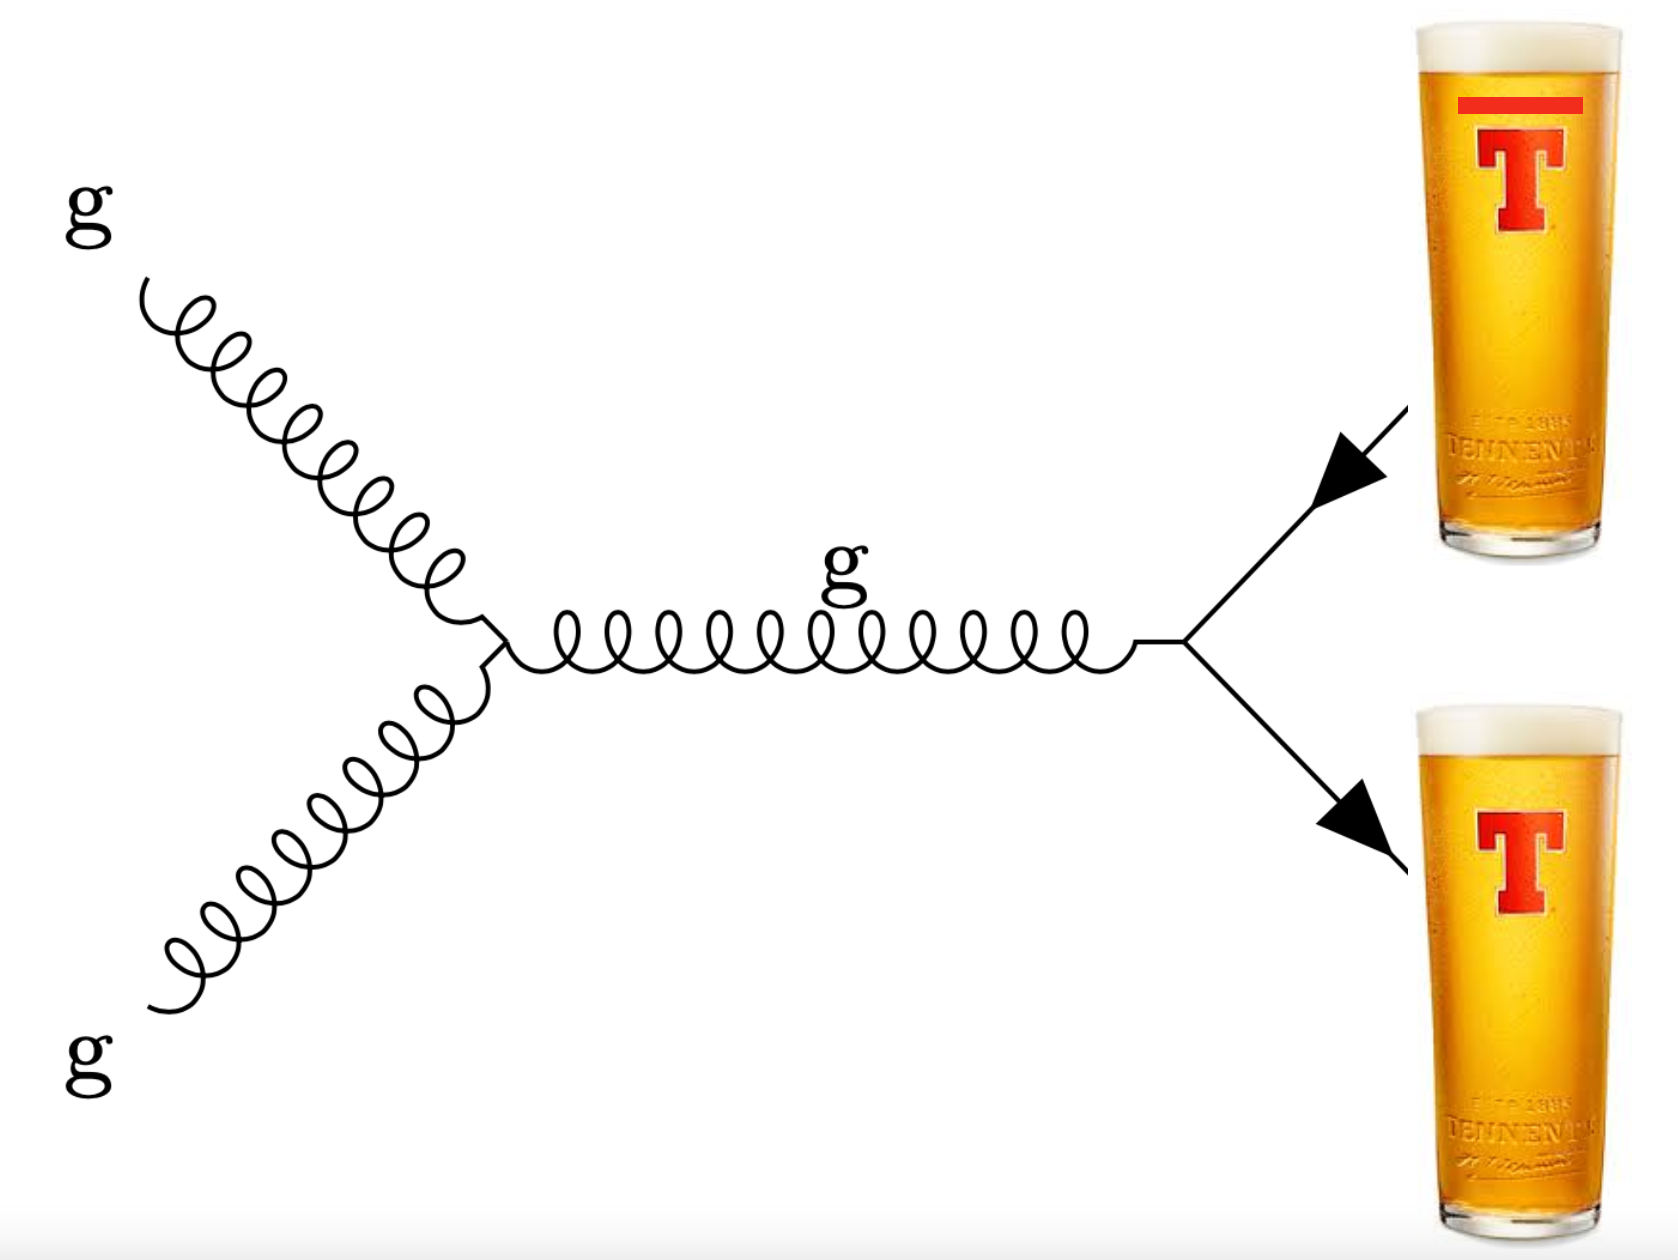
\includegraphics[width=0.75\linewidth]{Introduction/tennents_ttbar.png}
\caption[Short caption that shows up in list-of-figures]{Big caption what reads under the figure in the text}
\label{fig::example}
\end{figure}

%\end{document} % Depending on LaTeX setup this can be uncommented to compile chapters individually 

  %\documentclass[hyperpdf,nobind,twoside,hidefrontback]{hepthesis}  
%\newcommand*{\BASEPATH}{../} 
%\usepackage{xspace}
\usepackage{tikz}
\usepackage{morefloats,subfig,afterpage}
\usepackage{mathrsfs} % script font
\usepackage{verbatim}
\usepackage{cite}
%\usepackage{float} #For demanding figure is placed exactly where specified using H 
%\usepackage{multirow} #For multi-row tables 

%% Using Babel allows other languages to be used and mixed-in easily
%\usepackage[ngerman,english]{babel}
\usepackage[english]{babel}
\selectlanguage{english}

\graphicspath{{\BASEPATH figures/}{\BASEPATH tables/}}

%% High-energy physics stuff
%\usepackage{abhep}
\usepackage{hepnames}
\usepackage{hepunits}

% Definitely useful JJ macros
\usepackage{\BASEPATH JJthesis-defs}

%Tell TexCount to track red text seperately
%TC:newcounter RedText Problem Text
%TC:macro \col [RedText]

%Tell TexCount how to correctly account for macros: \macro #Words
%TC:macroword \ATLAS 1
%TC:macroword \ttbar 1
%TC:macroword \wdecay 2
%TC:macroword \wboson 2
%TC:macroword \mtop 1
%TC:macroword \mtopjet 2
%TC:macroword \zmumu 2
%TC:macroword \ljets 2
%TC:macroword \lpt 1
%TC:macroword \hpt 1
%TC:macroword \etmiss 1
%TC:macroword \HLTtap 1
%TC:macroword \frtwo 3
%TC:macroword \ISR 1
%TC:macroword \FSR 1
%TC:macroword \JSF 1
%TC:macroword \NDF 1
%TC:macroword \JSFdata 1
%TC:macroword \JSFsyst 1
%TC:macroword \JSFdatastat 1
%TC:macroword \jvt 1
%TC:macroword \nominal 2
%TC:macroword \mcatnlo 1
%TC:macroword \mcatnloX 1
%TC:macroword \phseven 2
%TC:macroword \AF 1
%TC:macroword \MC 1
%TC:macroword \RC 1
%TC:macroword \powheg 1
%TC:macroword \powhegbox 1
%TC:macroword \herwig 1
%TC:macroword \herwigseven 1
%TC:macroword \pythia 1
%TC:macroword \pythiasix 1
%TC:macroword \sherpa 1
%TC:macroword \evtgen 1
%TC:macroword \hathor 1
%TC:macroword \mgamc 1
%TC:macroword \madspin 1
%TC:macroword \openloops 1
%TC:macroword \openloopstwo 1
%TC:macroword \sherpaopenloops 2
%TC:macroword \mur 1
%TC:macroword \muf 1
%TC:macroword \muq 1
%TC:macroword \ttV 1
%TC:macroword \pThad 1
%TC:macroword \pTlep 1
%TC:macroword \pTttbar 1
%TC:macroword \HTfull 1
%TC:macroword \HTttbar 1
%TC:macroword \yhad 1
%TC:macroword \ylep 1
%TC:macroword \yttbar 1
%TC:macroword \mttbar 1
%TC:macroword \Naddjets 1
%TC:macroword \pTlead 1
%TC:macroword \pTsublead 1
%TC:macroword \dphileadhadtop 1
%TC:macroword \dphisubleadhadtop 1
%TC:macroword \dphilepbhadtop 1
%TC:macroword \dphittbar 1
%TC:macroword \dphileadsublead 1
%TC:macroword \mleadhadtop 1
%TC:macroword \Rleadhadtop 1
%TC:macroword \Rsubleadhadtop 1
%TC:macroword \arXivCode 1
%TC:macroword \CP 1
%TC:macroword \CPviolation 1
%TC:macroword \LHCb 1
%TC:macroword \LHC 1
%TC:macroword \LEP 1
%TC:macroword \CERN 1
%TC:macroword \bphysics 1
%TC:macroword \bhadron 1
%TC:macroword \Bmeson 1
%TC:macroword \bbaryon 1
%TC:macroword \Bdecay 1
%TC:macroword \bdecay 1



% Potentially useful Andy macros
% \DeclareRobustCommand{\parenths}[1]{\mymath{\left({#1}\right)}\xspace}
% \DeclareRobustCommand{\braces}[1]{\mymath{\left\{{#1}\right\}}\xspace}
% \DeclareRobustCommand{\angles}[1]{\mymath{\left\langle{#1}\right\rangle}\xspace}
% \DeclareRobustCommand{\sqbracs}[1]{\mymath{\left[{#1}\right]}\xspace}
% \DeclareRobustCommand{\mods}[1]{\mymath{\left\lvert{#1}\right\rvert}\xspace}
% \DeclareRobustCommand{\modsq}[1]{\mymath{\mods{#1}^2}\xspace}
% \DeclareRobustCommand{\dblmods}[1]{\mymath{\left\lVert{#1}\right\rVert}\xspace}
% \DeclareRobustCommand{\expOf}[1]{\mymath{\exp{\!\parenths{#1}}}\xspace}
% \DeclareRobustCommand{\eexp}[1]{\mymath{e^{#1}}\xspace}
% \DeclareRobustCommand{\plusquad}{\mymath{\oplus}\xspace}
% \DeclareRobustCommand{\logOf}[1]{\mymath{\log\!\parenths{#1}}\xspace}
% \DeclareRobustCommand{\lnOf}[1]{\mymath{\ln\!\parenths{#1}}\xspace}
% \DeclareRobustCommand{\ofOrder}[1]{\mymath{\mathcal{O}\parenths{#1}}\xspace}
% \DeclareRobustCommand{\SOgroup}[1]{\mymath{\mathup{SO}\parenths{#1}}\xspace}
% \DeclareRobustCommand{\SUgroup}[1]{\mymath{\mathup{SU}\parenths{#1}}\xspace}
% \DeclareRobustCommand{\Ugroup}[1]{\mymath{\mathup{U}\parenths{#1}}\xspace}
% \DeclareRobustCommand{\I}[1]{\mymath{\mathrm{i}}\xspace}
% \DeclareRobustCommand{\colvector}[1]{\mymath{\begin{pmatrix}#1\end{pmatrix}}\xspace}
 
%\begin{document}
% Uncomment to compile chapters individually
                                              
\chapter{\ATLAS Detector}
\label{chap::Detector}

\chapterquote{If we hit that bullseye the rest of the dominoes will fall like a house of cards. Checkmate!}%
{Captain Zapp Brannigan}

This is the chapter of my thesis all about the \ATLAS detector.

\section{Detector Hardware}
\label{sec::detector_hardware}
The \ATLAS detector\cite{ATLAS} has a $4\pi$ onion-like structure and some other stuff probably  


\section{Trigger System}
\label{sec::detector_trigger}
The trigger system allows interesting physics to be successfully extracted from the millions of interactions that occur at the \LHC at very high collision energies.

\subsection{Muon Trigger System}
\label{subsec::muon_trigger}
The muon trigger triggers on muons

%\end{document}
% Uncomment to compile chapters individually 

  \chapter{Theory}
\label{chap::Theory}

\chapterquote{you gonna eat that?}%
{Bennie the cat}

just talk about the most elegant marriage of mathematics and physics ever cooked up, no biggie.

\section{something about the standard model }
 
  %% To ignore a specific chapter while working on another, making the build faster, comment it out:
\end{mainmatter}

%% Produce the appendices
\begin{appendices}
  %% The "\appendix" call has already been made in the declaration
%% of the "appendices" environment (see thesis.tex).
\chapter{Pointless extras}
\label{app:Pointless}

\chapterquote{%
If the Flinstones' have taught us anything,\\ it's that pelicans can be used to mix cement.}%
{Homer Simpson -- 'Missionary Impossible'}

You can debate amongst yourselves on the necessity of appendices in a PhD thesis.

\section{Extra stuff, probably}
\label{app::Extras}
Here's a thing I did but in excruciatingly keen detail
\col{and this is some more red text}

%% Big appendixes should be split off into separate files, just like chapters
%\input{app-myreallybigappendix}

\end{appendices}

%% Produce the un-numbered back matter (e.g. colophon,
%% bibliography, tables of figures etc., index...)
\begin{backmatter}
  \begin{colophon}
  This thesis was made in \LaTeXe{} using the ``hepthesis'' class.
\end{colophon}

%% You're recommended to use the eprint-aware biblio styles which
%% can be obtained from e.g. www.arxiv.org. The file mythesis.bib
%% is derived from the source using the SPIRES Bibtex service.
\bibliographystyle{unsrt}
\bibliography{Bibliography/JJthesis.bib}

%% I prefer to put these tables here rather than making the
%% front matter seemingly interminable. No-one cares, anyway!
\listoffigures
\listoftables

%% If you have time and interest to generate a (decent) index,
%% then you've clearly spent more time on the write-up than the
%% research ;-)
%\printindex

\end{backmatter}

%% Close
\end{document}
